\graphicspath{{./Figs/}}


\chapter{Literature Review}
This chapter contains a review of the current literature published on MAV development and the extent to which propeller effects have been researched. It explores the effects that propellers have on MAVs, current research on non-linear lift distributions, separation bubbles and propeller interactions and effects.
%  Traditional methods of aircraft design have generally focused on larger aircraft \cite{Raymer2006} \cite{Roskam1989}.

\section{Proliferation of MAV's in the Aerospace Landscape}
\label{subsec:ProliferationMAVs}
Initially introduced during World War I, UAVs were heavily criticized due to inaccuracies and unreliability when performing missions. Few saw the potential and impact they could have in changing the landscape of a battlefield \cite{thebook}. UAVs have existed for centuries, although the modern era of UAVs commonly refers to the last four decades \cite{Cook2007}. 

It was not until Operation Desert Storm (1991) and the Balkan Peninsula conflict that the development and interest in UAVs took off \cite{thebook, MacConnell2007}.  The U.S. at the time saw a total income of \$2.27 billion dollars \cite{thebook} (a 9.5\% increase from the previous year of 1996). This marked a turning point in the the development of more complex UAVs \cite{tac2022} as the U.S. Department of Defense funded UAV research for the first time in 1996 \cite{keennon2003}. The recent shift to the miniaturisation of components, systems and aerial vehicles has already influenced the military sector \cite{Aleksander2018, Mil2022}, with several developments underway to reduce the visibility of reconnaissance aircraft and reduce the likelihood of aircraft being detected during missions \cite{Greenwood2019, Saytov2022}.  The most famous military MAV arguably being the Honeywell RQ-16 T-Hawk \cite{Agbeyangi2016}  which was mainly used by the U.S. forces in Iraq to search for roadside bombs \cite{Crivoi2022}. The success of which (largely due to its hovering feature) led the U.S. Navy to order a further 372 MAVs \cite{design2022}.

What started as a small initial interest in smaller and smarter drones has resulted in exponential growth in the sector \cite{NONAMI2007, Wang2019}. Technology improvements have led to the exponential growth in the capabilities of MAV seen today \cite{Yin2020, Jackson2016}. Where an initial drone supported only low camera resolution with meagre flight times, today incorporates several systems such as gyro stabilisation, GPS capability with way-point guidance, beyond the line of vision control, speeds of 70 km/h with a 30 minute flight time, and a 20-megapixel camera (DJI Phantom 4) \cite{Peppa2019}. 




% Look at section \ref{sec:ProliferationMAVs}.

\section{Limitations of MAV Design Techniques}
\label{subsec:Limitations}
While MAV technology is more accessible and viable to the mass market than it has ever been before \cite{Jackson2016}, there is no fully developed and validated way to optimize a MAV for a specified mission \cite{Bronz2009, HASSANALIAN2019}. Today, procedures involve developing a CAD model of the MAV or using software based on aerodynamics. This model is either then run through aerodynamic optimization software and/or tested in a wind tunnel to determine the main characteristics of the MAV \cite{Paulson2017}. The largest drawback of which is the lack of propeller effects accounted for, which are known to have a large effect on aerodynamics and stability \cite{Harikumar2021, Chinwicharnam2013}. MAV model tests have been conducted with a fixed position propeller \cite{Shams2020b, Durai2014}. Models are, however, typically tested without a spinning propeller, although these have been included in several aerodynamic software programs and specific tests \cite{Aboelezz2020}. 

However, a lack of validation from wind tunnel testing means that a full understanding of the effects a propeller has on MAVs has not been achieved. MAVs are small relative to the size of the propellers used. Hence, the propeller will significantly affect the stability, noise, overall endurance, performance and power consumption of a given MAV \cite{Shams2020, Chen2022}. 



\section{Low Reynolds Number Effects }\label{sec:Reynolds2}

% EXPLAIN HERE - what is RE
\label{sec:LowReynolds}
Due to the small size and Reynolds numbers at which MAVs operate (typically around Re=$10^5$ \cite{Huq2009} \cite{Winslow2018}), insects and other small animals are often studied to understand the flight dynamics which occur for small flying bodies \cite{Liu2009}. The Reynolds region in which MAVs typically fly is shown in Figure \ref{fig:MAVsizes}.

\begin{figure}[H]
% \hspace*{-1.3in}
  \centering
  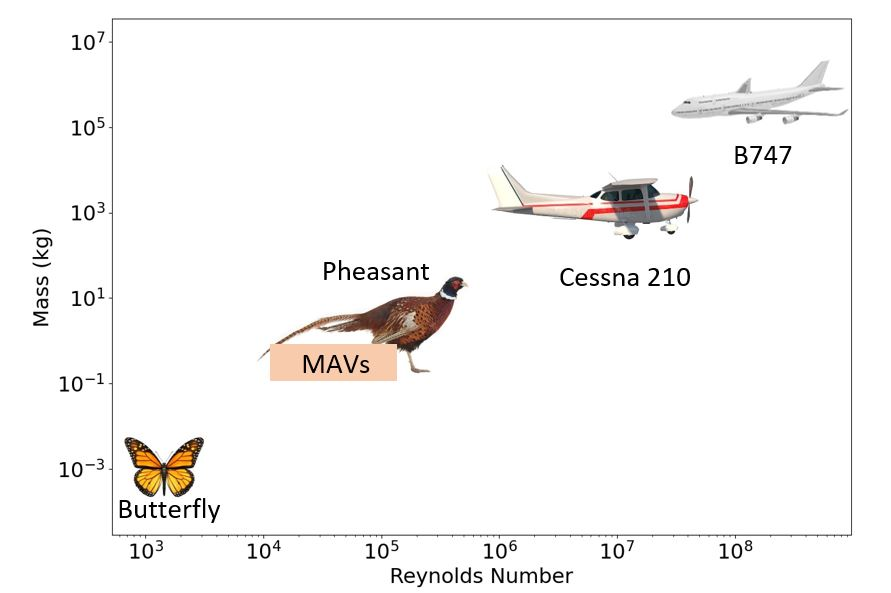
\includegraphics[width=\linewidth]{03_LiteratureReview/Figs/Reynolds.JPG}
  \caption{MAV speed with Reynolds number region in respect to flying bodies. Figure is adapted \cite{reynoldsFigure}. Image sources: \cite{butterfly, pheasant, cess, b474} }
  \label{fig:MAVsizes}
\end{figure}

 Null used wind tunnel tests to show that propellers on wings during low Reynolds flight increased the performance of the wing at high angles of attack \cite{Null2005}. Ananda also visualised this effect as shown in Figure \ref{fig:bladeslow}, however this is without the propeller being mounted on the wing directly.  

\begin{figure}[H]
% \hspace*{-1.3in}
  \centering
  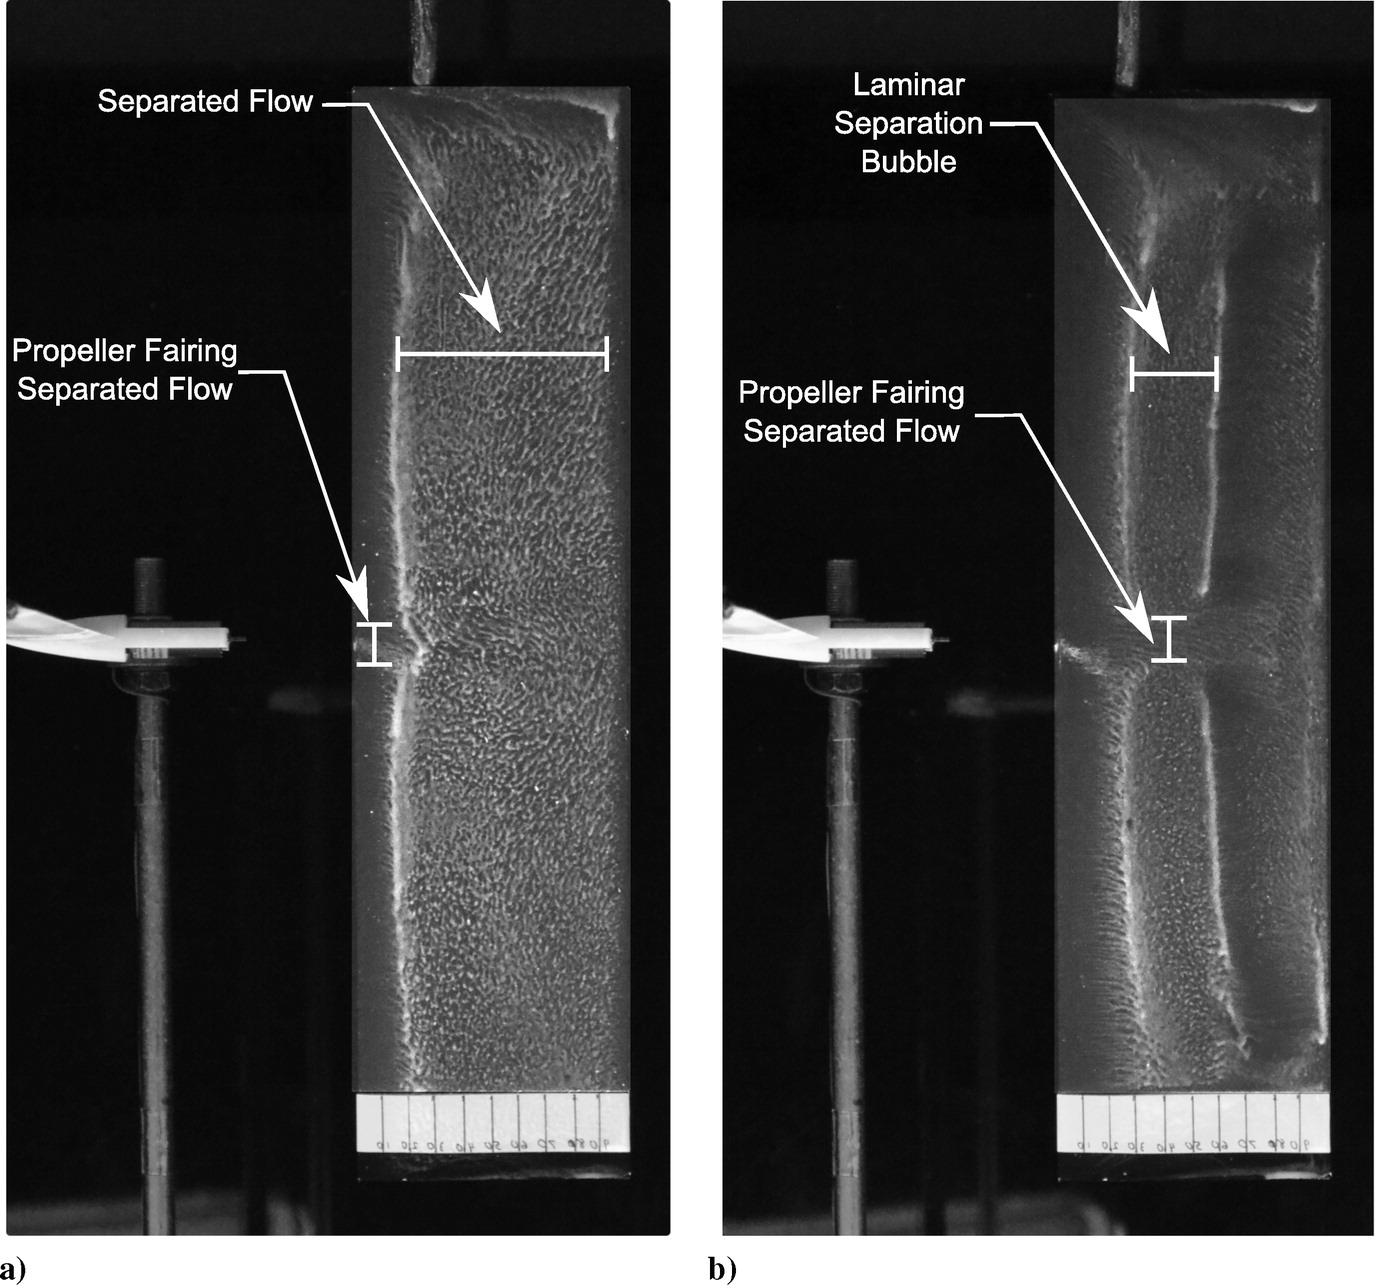
\includegraphics[width=0.8\linewidth]{03_LiteratureReview/Figs/blades.jpeg}
  \caption{Flow characteristics across the propeller when the propeller is turned off (a) and when the propeller is turned on (b) \cite{Ananda2018}}
  \label{fig:bladeslow}
\end{figure}



% \begin{figure}[H]
% \hspace*{-1.3in}
%   \centering
%   \includegraphics[width=\linewidth]{03_LiteratureReview/Figs/285202324_1193411864727797_5746060971373574289_n.png}
%   \caption{MAV speed with Reynolds number region in respect to flying bodies \cite{reynoldsFigure}}
%   \label{fig:MAVsizes}
% \end{figure}

Low Reynolds number compressible aerodynamics are particularly important for small aircraft. Aircraft used to survey martian terrain and MAVs are mainly influenced due to the change in atmosphere and small geometry respectively \cite{Munday2015}. Low Reynolds number effects are critical for propeller based MAV systems. As the root and tip of a propeller can differ significantly in Mach number \cite{Munday2015}. As MAVs have small ARs due to their smaller size and non-conventional structures, low AR wings at low Reynolds numbers have recently, in particular, been studied \cite{Bhat2019} \cite{Torres2012}. Cosyn showed that the flow over these is characterised by complex 3D phenomena such as wing-tip vortices, laminar to turbulent transitions, and flow separation, and re-attachment \cite{Cosyn2012}.

Airfoils in particular have been investigated due the importance of their use in aircraft. At low Reynolds numbers (10,000 < Re < 50,000) the flow remains laminar when the airfoil is aligned with the incoming flow. Pressure gradients created due to a larger angle of attack or high camber (airfoil thickness) create turbulent flow following separation. This is also shown in Figure \ref{fig:Re3}. Early research by Mueller showed that the maximum lift coefficient is typically 0.5 for airfoils before stalling at low Reynolds numbers \cite{Mueller1985}. \\
At Reynolds numbers from 50,000 to 100,000 the separation bubble and turbulent layer thickness increase in size \cite{Winslow2018}. The separated shear layer will eventually gain enough momentum from the free-stream in order to reattached to the airfoil as shown in Figure \ref{fig:Re3}. The separation bubble is also known as a laminar separation bubble (LSB). Mueller found that airfoil choice in this region was critical to the aerodynamic performance. Airfoils with large camber (thickness) produce large pressure gradients causing separating which leds to the formation of LSBs on the upper surface of the wing \cite{Mueller1985}. As Reynolds numbers increases the separation and attachment move towards the leading edge \cite{Winslow2018}. The turbulent layer thickess reduces and the airfoil performance improves. The turbulent layer thickness varies between airfoils and LSBs can still form up until around a Reynolds number of 200,000. This is notable as most MAVs operate around the 50,000 to 200,000 Reynolds number range \cite{Cosyn2006}. At Reynolds numbers greater than 500,000 the separation point generally lies on the leading edge. The performance of airfoils increases due to the reduced turbulent layer \cite{Winslow2018}. %Separation however can occur at high angles of attack. Turbulent boundary layer initially separates from the tailing edge but this separation will move towards the leading edge as the angle of attack increases. This can lead to stall of the entire airfoil \cite{Winslow2018}. 

\begin{figure}[H]
    \centering
    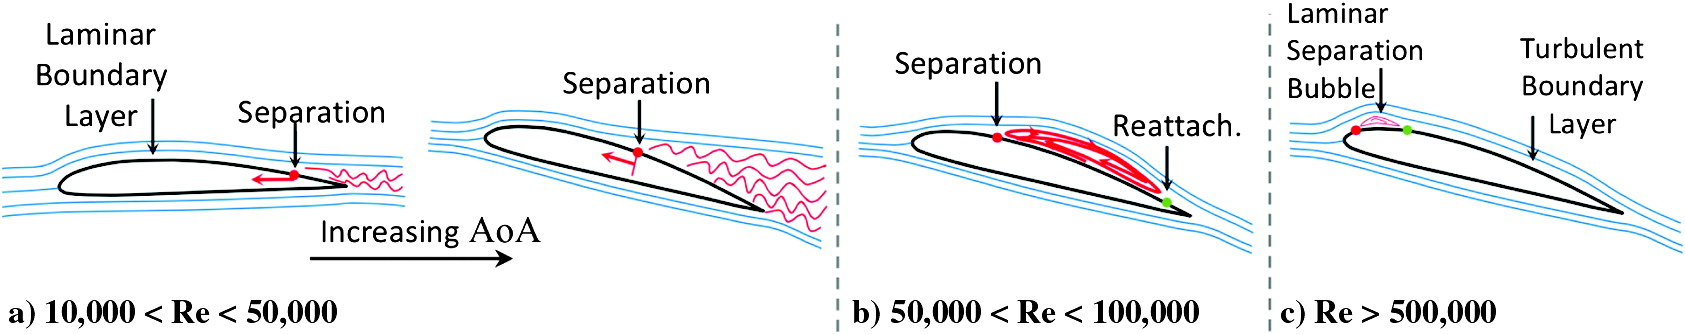
\includegraphics[width = \linewidth]{02_Background/Figs/airfoil.jpeg}
   \caption{Flow separation position change with Reynolds number \cite{Winslow2018}}
    \label{fig:Re3}
\end{figure}

\subsection{Laminar Separation Bubbles and Vortices}
Flow separation and re-attachment create separation bubbles over wings and account for the most drag over the surface of wings at these low Reynolds numbers \cite{ravi}. LSBs typically occur at Reynolds number below 200,000. Perot showed how in the presence of adverse pressure gradients, airflow separates from the wing \cite{Perot1999}. This was further validated by Mohamed \cite{Mohamed2014}. Mohamed investigated these LSBs and showed that they can deteriorate a MAVs stability as the drag induced by these bubbles leads to a low-pressure region over the bubbles, causing severe perturbations of motion \cite{Mohamed2014}. Marxen found these bubbles are typically stable, as no transfer of energy occurs between the flow circulating inside the bubble and the laminar flow, which passes over the top \cite{Marxen2010}. Detailed anatomy of how LSBs affect flow over a typical airfoil shape is shown in Figure \ref{fig:Laminar}.

% CITE ISSUETODO

\begin{figure}[H]
% \hspace*{-1.3in}
  \centering
   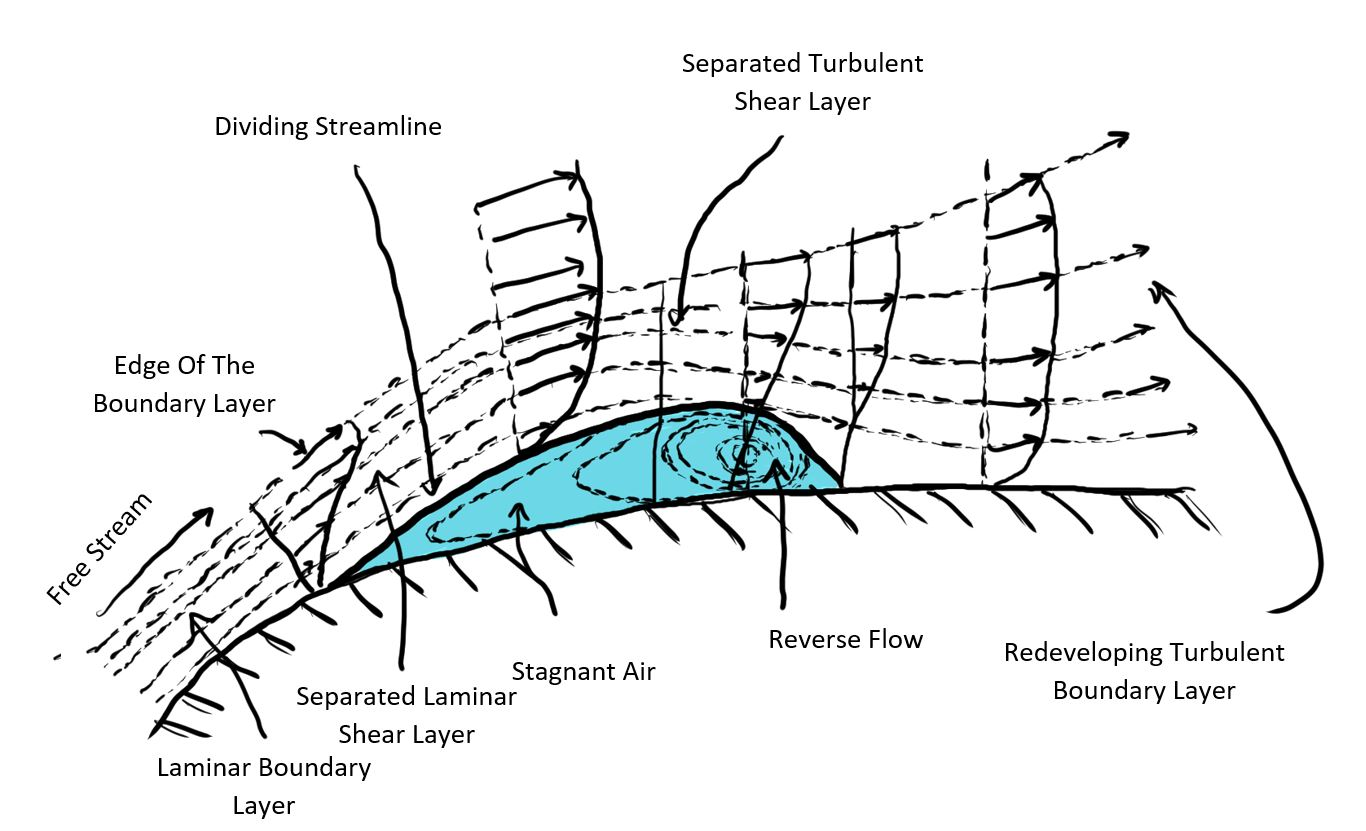
\includegraphics[width=\linewidth]{03_LiteratureReview/Figs/LSB.jpg}
  \caption{Anatomy of laminar separation bubbles. Figure adapted from Mohamed \cite{Mohamed2014}}
  \label{fig:Laminar}
\end{figure}

Crimi then investigated the implications of this separation when varying the angle of attack. Crimi determined that the angle of attack of an airfoil affects the placement of LSBs. When the angle of attack suddenly increases (e.g. during a gust), a separation of the shear layer is also seen close to the leading edge \cite{Crimi1976}. Mohamed explains this as the shear layer transitioning earlier due to this disturbance  \cite{Mohamed2014}. Additionally, LSBs and vortices also significantly affect the coefficient of lift ($C_L$) of an airfoil. $C_L$ is affected to a greater extent in smooth flow conditions as more suction is experienced inside an LSB with a smooth surface.


% \begin{figure}[H]
%      \centering
%      \begin{subfigure}[b]{\textwidth}
%          \centering
%          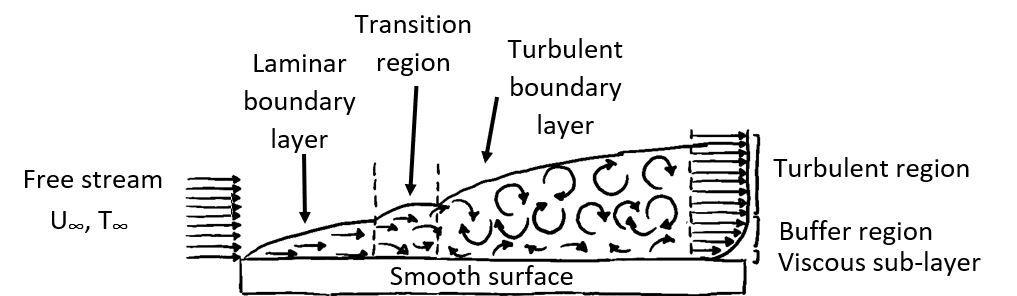
\includegraphics[width=\textwidth]{02_Background/Figs/smooth.JPG}
%          \caption{Smooth surface}
%          \label{fig:Pressoo2a}
%      \end{subfigure}
%      \hfill
%      \begin{subfigure}[b]{\textwidth}
%          \centering
%          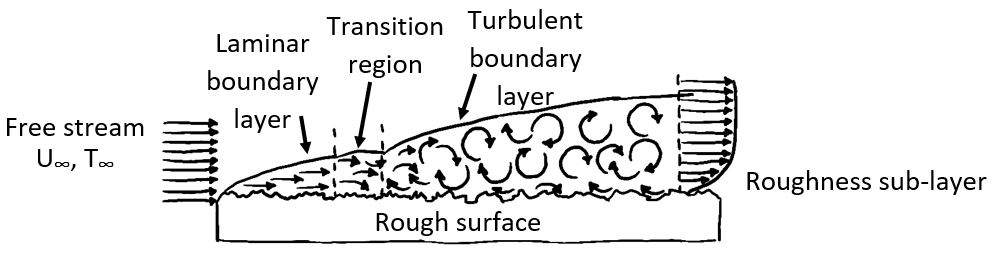
\includegraphics[width=\textwidth]{02_Background/Figs/rought.JPG}
%          \caption{Rough surface}
%          \label{fig:Pressoo2b}
%      \end{subfigure}
%      \hfill
%          \caption{a) Laminar flow to turbulence without surface roughness. b) Smaller transition region and turbulent boundary layer length with a rough surface. Figure is adapted \cite{Choi2006}.}
%   \label{fig:compare}
% \end{figure}


Mohammed found this larger suction seen on smooth surfaces, induces pitching and rolling moments \cite{Mohamed2014}. In the stall region angle of attack, turbulent flow results in a higher lift. The opposite is true for smooth flow. Turbulence could therefore increase the characteristic airfoil performance at low Reynolds numbers \cite{Mohamed2014}. These characteristics are also shown in Figure \ref{fig:flow}.


\begin{figure}[H]
     \centering
     \begin{subfigure}[b]{0.45\textwidth}
         \centering
         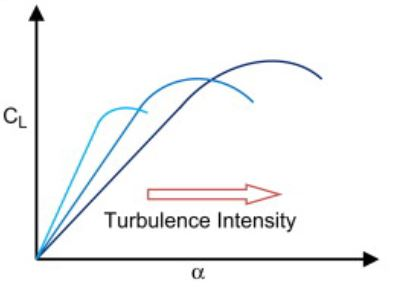
\includegraphics[width=\textwidth]{03_LiteratureReview/Figs/acondition.JPG}
         \caption{Turbulence Intensity with lift curve}
         \label{fig:P2a}
     \end{subfigure}
     \hfill
     \begin{subfigure}[b]{0.45\textwidth}
         \centering
         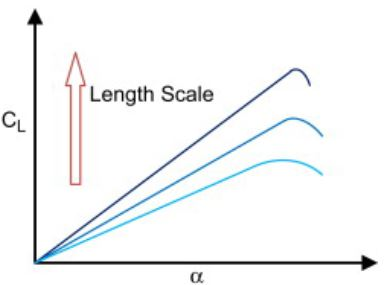
\includegraphics[width=\textwidth]{03_LiteratureReview/Figs/bcondition.JPG}
         \caption{Length scale with lift curve}
         \label{fig:P2b}
     \end{subfigure}
     \hfill
          \caption{Airfoil aerodynamic performance variation with increasing: (a) turbulence intensity (b) length scale \cite{Mohamed2014}}
        \label{fig:flow}
\end{figure}





Investigations using materials with varying roughness have also been used to induce this transition to turbulent flow. Choi investigated this transition with some results shown in Figure \ref{fig:rough}. These show that the LSBs are reduced in the flow over airfoils when moving over a rough surface.

% ISSUE
\begin{figure}[H]
     \centering
     \begin{subfigure}[b]{0.45\textwidth}
         \centering
         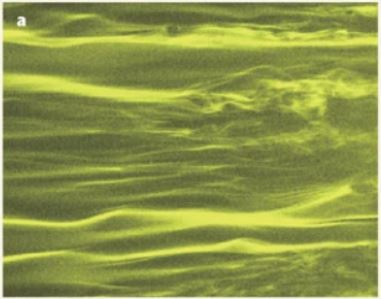
\includegraphics[width=\textwidth]{03_LiteratureReview/Figs/a2.JPG}
         \caption{Smooth surface}
         \label{fig:Ps2a}
     \end{subfigure}
     \hfill
     \begin{subfigure}[b]{0.45\textwidth}
         \centering
         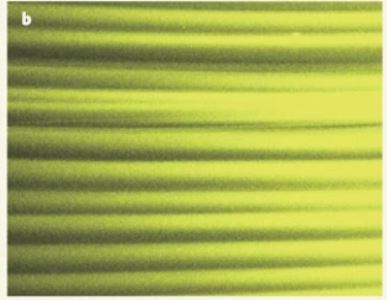
\includegraphics[width=\textwidth]{03_LiteratureReview/Figs/b2.JPG}
         \caption{Rough surface}
         \label{fig:Ps2b}
     \end{subfigure}
     \hfill
           \caption{Flow patterns shown by smoke. Laminar flow to turbulence without surface roughness (a). Laminar flow for with a rough surface (b).  \cite{Choi2006}}
  \label{fig:rough}
\end{figure}







% Modelling LSBs and vortices in software is a difficult challenge and software such as Xfoil are unable to account for concepts such as the 'bursting of laminar bubble' which is a concept in which the free-stream airflow does not reattach to the airfoil. 

\subsection{Non-Linear Lift Distribution}


\label{sec:Non-Linear Lift Distribution}
Early on in the study of aerodynamics, theories developed from the study of conventional aircraft were applied to the bodies of small flying objects and animals such as birds. Traditional aerodynamic theories provide good results and insights when steady flows move across a stationary body. As mentioned by Roccia, they could not however, explain what allows small insects and birds to fly, leading to the paradox of "a bee cannot fly" \cite{bees} \cite{Roccia2016}. Roccia determined that the issue lies in the fact that non-linear and steady flows mainly characterize the flight of biological creatures \cite{Roccia2016}. This non-linear lift distribution is primarily caused by the low Reynolds number that these small bodies fly at and the low AR that MAV aircraft typically have (AR < 3).

 Early experimental work conducted by Winter showed that wings with small ARs can be described with a bound vortex flow and a wing-tip flow, which is also known today as vortices \cite{H1936}. Wingtip vortices are particularly important, and even in general aircraft, lead to regulations such as spacing rules between aircraft and aerodynamic noise \cite{Qin2021}. At the wingtips the pressure difference between the upper and lower surface cause a swirling vortex when in a free stream flow. This phenomenon is also shown in Figure \ref{fig:vortex}. Cosyn and Vierendeels showed that this creates a low pressure cell at the wing tip which deforms the lift distribution in this region \cite{Cosyn2006}. 
 
 \begin{figure}[H]
% \hspace*{-1.3in}
  \centering
  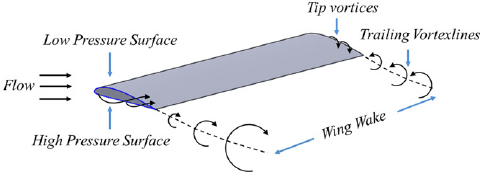
\includegraphics[width=\linewidth]{03_LiteratureReview/Figs/Development-of-wingtip-vortices-over-a-wing-section.png}
  \caption{ Development of wingtip vortices over a wing section 
 \cite{Kumar2015}}
  \label{fig:vortex}
\end{figure}

 Zimmerman showed that the wing-tip geometry influences the aerodynamic performance for low AR wings \cite{Zimmerman1936}. Zimmerman also concluded that in order to produce the same coefficient of lift for lower AR wings, a higher angle of attack is required \cite{Zimmerman1936}. Low AR wings are also more susceptible to instability caused by disturbances \cite{DeVoria2017}. Watkins showed that a sideslip is easily induced by a slight wind gust for low AR aircraft \cite{Watkins2012}. Shields investigated the inherent stability modes of low AR wings, determining that low AR wings have near-zero roll damping \cite{Shields2015}. This means that roll moments created by flow asymmetries have a significant impact on low AR aircraft \cite{Shields2015}.
 
 Mueller and DeLaurier found that for low AR aircraft, the center of lift was also sensitive to the angle of attack \cite{Mueller2003}. This is due to the wingtip vortices increasing with angle of attack. Therefore the non-linear aerodynamics dominate more at higher angle of attack, Pelletier also determined that these effects are more pronounced for low AR aircraft \cite{Pelletier2012}. 


\section{Propeller Wing Interaction}\label{sec:propellerWingInteraction}




Propellers are commonly mounted on wings and significantly alter the flow seen over airfoils. Prandtl first studied the propeller-wing interaction at the start of the last century. The results concluded that two main effects impact the wing and flow behaviour. The first is due to the swirling of the propeller, which creates an ever-varying velocity. The second is due to an increase in inflow velocity \cite{Pant}. Mounting propellers on the tips of the wing has also been shown to have benefits to performance compared with other wing positions \cite{Miranda1986}. Miranda found that substantial performance improvements can be achieved by properly mounting propellers on the wingtips of wings \cite{Miranda1986}, this was also further validated by Sinnige \cite{Sinnige2019} and other teams \cite{Veldhuis2000} \cite{review}. 

Numerical analysis by Rizk using the Vortex Lattice Method has also validated these observations \cite{Rizk2012}. Veldhuis found that propellers have a higher axial velocity at the blade tip than where it is joined at a hub \cite{Veldhuis2000}. Ferraro also determined that the slipstream created by the propeller can be split into the axial, and tangential velocity components \cite{Ferraro2014}. The tangential velocity component accounts for the dynamic pressure across the wing \cite{Ferraro2014}. The swirl is anti-symmetrical and changes the incoming flow that the wing sees. This is also shown in Figure \ref{fig:2a} \cite{Ferraro2014}. The axial velocity affects the dynamic pressure on the wing. The axial velocity is considered to be symmetric when the propeller flow is uniform and undisturbed, as shown in Figure \ref{fig:2b} \cite{Ferraro2014}.


\begin{figure}[H]
     \centering
     \begin{subfigure}[b]{0.4\textwidth}
         \centering
         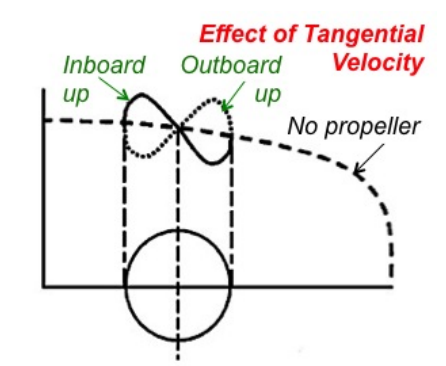
\includegraphics[width=\textwidth]{03_LiteratureReview/Figs/tanget.png}
         \caption{Tangential propeller effects}
         \label{fig:2a}
     \end{subfigure}
     \hfill
     \begin{subfigure}[b]{0.4\textwidth}
         \centering
         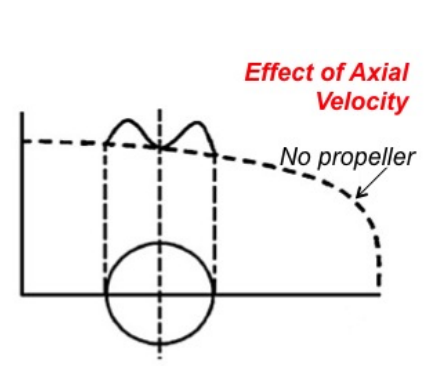
\includegraphics[width=\textwidth]{03_LiteratureReview/Figs/axial.png}
         \caption{Axial propeller effects}
         \label{fig:2b}
     \end{subfigure}
     \hfill
        \caption{Tangential and Axial velocity effects \cite{Ferraro2014}}
        \label{fig:prop}
\end{figure}


\begin{figure}[H]
% \hspace*{-1.3in}
  \centering
  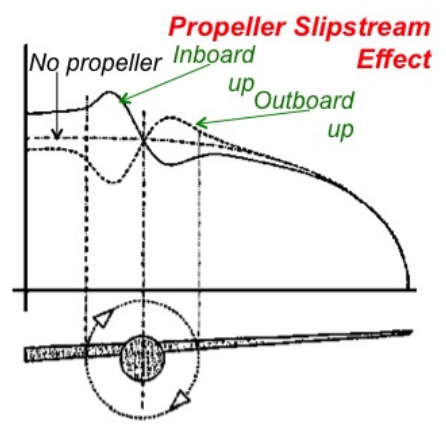
\includegraphics[width=0.4\linewidth]{03_LiteratureReview/Figs/slipstream.png}
  \caption{ Propeller slipstream effects on a finite wing \cite{Ferraro2014}}
  \label{fig:overallProp}
\end{figure}

As the dynamic pressure increases, a gain in lift coefficient is seen as shown in Figure \ref{fig:propanswer}. This increase in lift coefficent is also partially due to the lack of separation seen when increasing the revolutions per minute (RPM) of the propeller. Shams shows that this leads to a forward shift in the aerodynamic center of the aircraft \cite{Shams2020} \cite{Shams2020b}.


\begin{figure}[H]
% \hspace*{-1.3in}
  \centering
  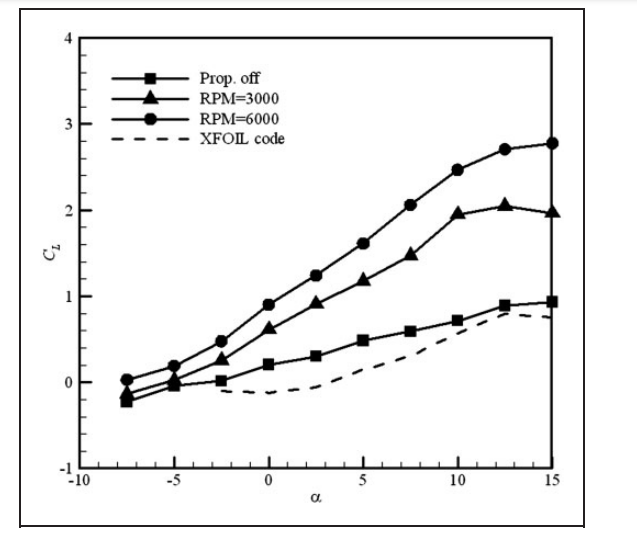
\includegraphics[width=0.8\linewidth]{03_LiteratureReview/Figs/Cl.png}
  \caption{ Effect of propeller slipstream on the lift coefficient
curve with angle of attack (Re =0.3 x $10^5$
) \cite{Aminaei2019}.}
  \label{fig:propanswer}
\end{figure}


The slipstream effect is shown in Figure \ref{fig:peoptoyou}. The inboard wing sees a higher angle of attack, and hence an up-wash effect is seen (y/b $>$ 0). Aminaei found that in the propeller down-wash region (y/b $<$ 0) a delay is experienced in the flow transition than when compared with the up-wash region \cite{Aminaei2019}. This is due to the reduced local angle of attack on the wing, which moves the transition region towards the trailing edge. These effects can also affect the flow stream beyond the propeller and lead to non-linear lift distributions further from the propeller as well. 
 
\begin{figure}[H]
% \hspace*{-1.3in}
  \centering
  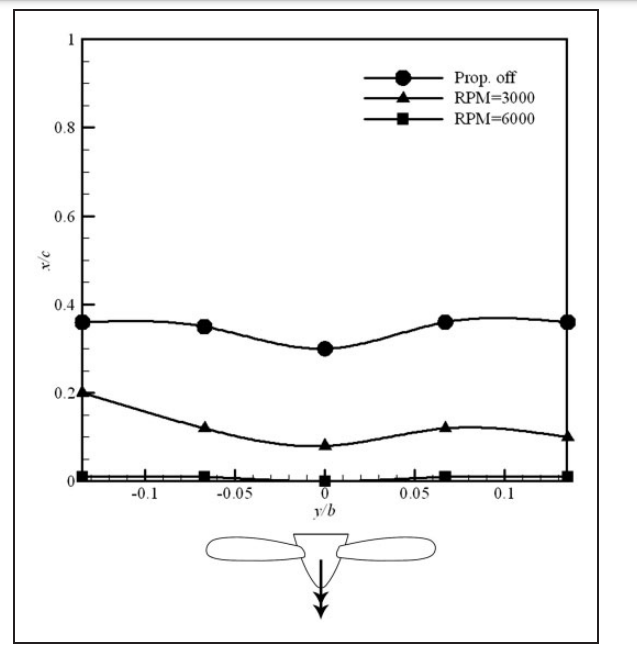
\includegraphics[width=0.8\linewidth]{03_LiteratureReview/Figs/propeller effects.png}
  \caption{Propeller slipstream effect with span-wise location for airflow transition over the wing upper surface, $\alpha = 2.5 ^\circ$ \cite{Aminaei2019}.}
  \label{fig:peoptoyou}
\end{figure}

    Prantl was one of the first to investigate the influence of propellers on wings \cite{Prandtl1931} and Franke and Weinig one of the first to investigate the rotational velocity's effects on the lift distribution across the wing \cite{Franke1939}. Framk and Weinig showed that the circulation distribution in regards to the slipstream can be predicted and used the lifting line theory in order to prove this \cite{Franke1939}. Jameson went on to develop simple equations to quantify the lift and drag of wings in jet slipstreams \cite{Jameson1970}. Ellis devloped programs to run multiple lifting line approximations in order to quanitfy the circulation pattern, when propeller effects are being accounted for \cite{Ellis1971}. These approximations however, were all too rudimentary and could not be used to predict the flow characteristics over wings. Several models and equations to represent these effects have been created. Veldhuis concluded that the propeller effects can only be described completely when using the Full Interaction Mode (FIM) \cite{Veldhuis2004}. 

% Up to Veldhuis

Veldhuis also determined that there are four main regions of influence which the propeller has. These proposed sections are not independent of each other but rather act as a smooth transition from one to the other \cite{Veldhuis2004}. As shown in Figure \ref{fig:propfour} the local blade angle of attack increases where the blade move down (P-II in Figure \ref{fig:propfour}) and decreases where the blade moves up (P-IV in Figure \ref{fig:propfour}). The induced angle of attack is visualised in Figure \ref{fig:propangles}. The effect of the propeller to induce this change in effective angle of attack is most greatly seen when the propeller is parallel to the wing span \cite{Veldhuis2004}.

\begin{figure}[H]
% \hspace*{-1.3in}
  \centering
  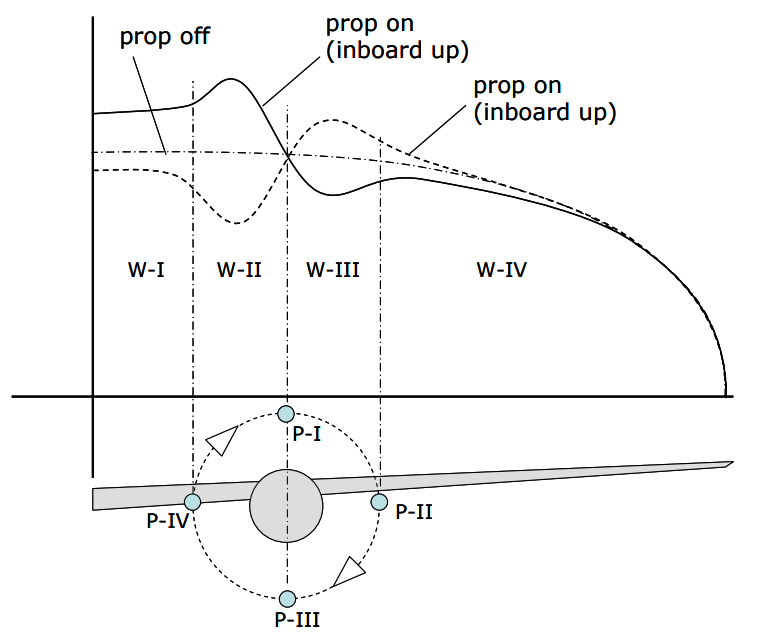
\includegraphics[width=0.8\linewidth]{03_LiteratureReview/Figs/four.png}
  \caption{Influence areas related to propeller-wing interaction based on the loading distributions \cite{Veldhuis2004}}
  \label{fig:propfour}
\end{figure}

\begin{figure}[H]
% \hspace*{-1.3in}
  \centering
  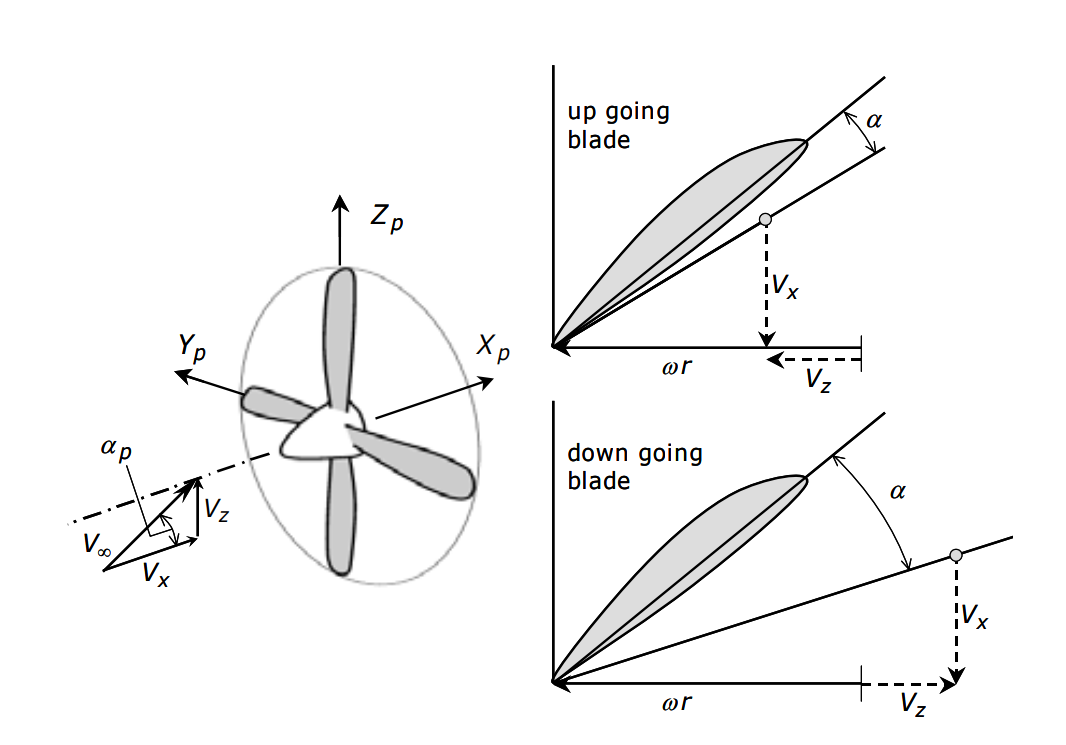
\includegraphics[width=0.8\linewidth]{03_LiteratureReview/Figs/anlges.png}
  \caption{Blade angle of attack variation due to propeller pitch angle \cite{Veldhuis2004}}
  \label{fig:propangles}
\end{figure}

Veldhuis also found that the extent of the swirl relaxation is dependent on the propellers position, free stream conditions and the overall wing loading \cite{Veldhuis2004}. A more recent study by Veldhuis simulated these effects through the use of CFD \cite{Veldhuis2016}. Ananda also concludes that for the tractor configuration, in a low speed wind tunnel, the flow transistions to turbulent flow earlier. This reduces the drag and increases the lift to drag ratio. These benefits were not seen when analysing the pusher configuration.












%Tractor/pusheer mounted





% \cite{Harikumar2021} Shams investigated the left turning tendencies of right-handed propellers \cite{Shams2020} \cite{Chen2022} \cite{Aminaei2018} \cite{Null2005} \cite{Parga2007}  \cite{Jana2020}. 

\subsection{Stability Effects}
As propellers have been shown to have a strong influence on the lift distribution across wings, the overall lateral and longitudinal stability will be affected. Shams has showed that increasing the propeller diameter and RPM increase the moment produced creating a larger pitching moment on the aircraft \cite{Shams2020}. Tractor configurations have also been investigated by Shams. The tractor configuration creates an increase in the rolling and yaw moments acting on the aircraft \cite{Shams2020}. Propellers do also produce a torque effect, further destabilizing the aircraft by creating a asymmetric roll. 

\subsection{Aerodynamic Parameters}
\label{sec:AerodynamicParameters}
The characteristics of an aircraft are given by a combination of the aerodynamic parameters that describe it. For MAV, this is more complex as these aircraft do not allow for the same assumptions to be made in calculations. New methods such as those developed by Shen, for determining the aerodynamic parameters are currently being developed, and proposed in order to address these differences \cite{Shen2018, Roberts2011}. Aerodynamic forces are crucial to the overall design of any aircraft \cite{Aero2012}. In order to determine these forces for MAVs, a variety of techniques have been used, such as the Athena Vortex Lattice Method used by Stewart and Hrad \cite{Stewart2007, Hrad2010}. However, this method cannot predict the separation of flow as the lift is assumed to increase linearly with the angle of attack.  This is not the case at low Reynolds numbers \cite{Zhang2022}. Aboelezz outlines a process in which a fixed-wing MAV can be designed, whereby he uses physical wind tunnel testing in order to evaluate the MAVs actual flight performance \cite{Aboelezz2020}. Bollay and Belotserkovskii have both proposed modified versions of Prandtl's lifting line theory \cite{Bollay1939, Belotserkovskii1968}, though validations with experimental data are limited in scope and do not validate propeller-wing interactions.

\subsection{The General Micro Aerial Vehicle}
\label{subsec:GenMAV}
Today the interest, research and development of MAVs are continually increasing. However, in order to focus on particular aspects or compare various designs, a "baseline" geometry is required. An example of this is the GENMAV developed by Stewart \cite{Stewart2007} shown in Figure \ref{fig:genmav2}.

\begin{figure}[H]
    \centering
    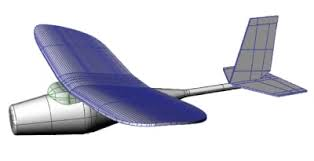
\includegraphics[width=0.8\linewidth]{04_Progress/Figs/genMav.jpeg}
    \caption{GenMAV Model \cite{Stewart2007}}
    \label{fig:genmav2}
\end{figure}

While there are various models which have been tested to determine the main aerodynamic properties \cite{Stewart2007} \cite{Aboelezz2020}, none have completed a physical wind tunnel test while accounting for the effects of a powered propeller. Initial GENMAV aerodynamic data was determined by using the vortex-panel method by Stewart \cite{Stewart2007}, and did not involve wind tunnel testing. The effects of propeller induced flow have also been studied for both fixed and free-spinning propellers, but currently, no data is available for wind tunnel tests of a powered propeller MAV.

\subsection{Optimization Techniques and Validation}
\label{subsec:Optimization}
Many non-standard aircraft designs are evaluated using software to analyse aerodynamic characteristics and then optimised through a variety of typical software engineering methods such as the particle swarm method used by Gomez to optimize the algorithm for the attitude and altitude, and Boutemedjet who used this to optimize the wing planform parameters of a MAV \cite{Gomez2020, Boutemedjet2019}. These procedures are used, as non-standard aircraft designs are more tedious to design and even more complex to set up and test than standard aircraft designs. The unique constraints that MAVs have and how they led to poor attitude control are shown in Figure \ref{fig:MAVconstrain}.

\begin{figure}[H]
% \hspace*{-1.3in}
  \centering
   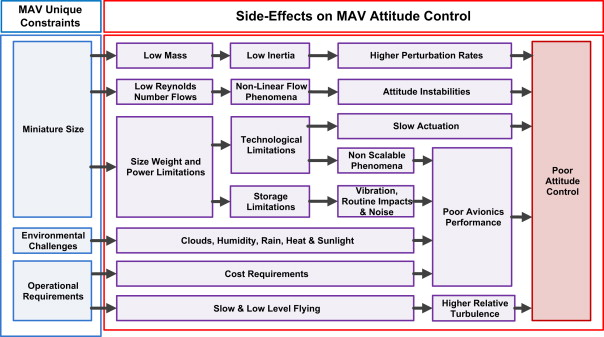
\includegraphics[width=\linewidth]{03_LiteratureReview/Figs/fowchart.jpg}
  \caption{Unique constraints of MAVs \cite{Mohamed2014}}
  \label{fig:MAVconstrain}
\end{figure}

Mohamed found that the physical size, environment and flight regime have strong effects on a MAVs ability to fly and carry payloads \cite{Mohamed2014}. Many groups of researchers have created software to optimize MAVs by using optimization algorithms such as genetic algorithms, non-dominating sorting generic algorithms, particle swarm optimization and sequential quadratic optimization programs. While some have accounted for low speed flight \cite{Vijayanandh2019, Bronz2009, HASSANALIAN2019}, no optimization techniques accounting for propeller-interaction effects currently exist. Many investigations into propeller effects show the propeller has significant effects on wing aerodynamics, both in regards to performance and also stability \cite{Parga2007, Jana2020}. None have been used with the results of spinning propellers in physical wind tunnel testing. Therefore these software models are currently invalid when also accounting for propeller-wing effects.

%  \cite{Harikumar2021} \cite{Shams2020b} \cite{Chen2022} \cite{Aminaei2018} \cite{Null2005}

